%%%%%%%%%%%%%%%%%%%%%%%%%%%%%%%%%%%%%%%%%
% baposter Portrait Poster
% LaTeX Template
% Version 1.0 (15/5/13)
%
% Created by:
% Brian Amberg (baposter@brian-amberg.de)
%
% This template has been downloaded from:
% http://www.LaTeXTemplates.com
%
% License:
% CC BY-NC-SA 3.0 (http://creativecommons.org/licenses/by-nc-sa/3.0/)
%
%%%%%%%%%%%%%%%%%%%%%%%%%%%%%%%%%%%%%%%%%

%----------------------------------------------------------------------------------------
%	PACKAGES AND OTHER DOCUMENT CONFIGURATIONS
%----------------------------------------------------------------------------------------

\documentclass[a1paper,portrait,fontscale=0.418]{baposter}

\usepackage[font=small,labelfont=bf]{caption} % Required for specifying captions to tables and figures
\usepackage{booktabs} % Horizontal rules in tables
\usepackage{relsize} % Used for making text smaller in some places
\usepackage{amsmath}
\usepackage{amsfonts}
\usepackage{amssymb}
\usepackage{amsthm}
\usepackage{algorithm2e}
\usepackage{listings}
\usepackage{xcolor}
\usepackage{tikz}
\usepackage{booktabs}
\usepackage{subfigure}
\usepackage[english]{babel}
\usepackage{blindtext}

\usepackage{tikz}
\usepackage{tikz-uml}
\tikzumlset{fill class=white}


\lstdefinelanguage{JavaScript}{
  keywords={typeof, new, true, false, catch, function, return, null, catch, switch, var, if, in, while, do, else, case, break},
  keywordstyle=\color{blue}\bfseries,
  ndkeywords={class, export, boolean, throw, implements, import, this},
  ndkeywordstyle=\color{darkgray}\bfseries,
  identifierstyle=\color{black},
  sensitive=false,
  comment=[l]{//},
  morecomment=[s]{/*}{*/},
  commentstyle=\color{purple}\ttfamily,
  stringstyle=\color{red}\ttfamily,
  morestring=[b]',
  morestring=[b]"
}
\lstset{
   language=JavaScript,
   %backgroundcolor=\color{lightgray},
   extendedchars=true,
   basicstyle=\footnotesize\ttfamily,
   showstringspaces=false,
   showspaces=false,
   numbers=left,
   numberstyle=\footnotesize,
   numbersep=9pt,
   tabsize=2,
   breaklines=true,
   showtabs=false,
   captionpos=b
}

\newcommand{\js}[1]{\lstinline[language=Javascript]$#1$}


\graphicspath{{figures/}} % Directory in which figures are stored

\definecolor{bordercol}{RGB}{40,40,40} % Border color of content boxes
\definecolor{headercol1}{RGB}{240,240,240} % Background color for the header in the content boxes (left side)
\definecolor{headercol2}{RGB}{80,80,80} % Background color for the header in the content boxes (right side)
\definecolor{headerfontcol}{RGB}{0,0,0} % Text color for the header text in the content boxes
\definecolor{boxcolor}{RGB}{255,255,255} % Background color for the content in the content boxes


\begin{document}

\background{ % Set the background to an image (background.pdf)
\begin{tikzpicture}[remember picture,overlay]
\draw (current page.north west)+(-2em,2em) node[anchor=north west]
{
\includegraphics[height=1.1\textheight]{background.pdf}};
\end{tikzpicture}
}

\begin{poster}{
grid=false,
borderColor=bordercol, % Border color of content boxes
headerColorOne=headercol1, % Background color for the header in the content boxes (left side)
headerColorTwo=headercol2, % Background color for the header in the content boxes (right side)
headerFontColor=headerfontcol, % Text color for the header text in the content boxes
boxColorOne=boxcolor, % Background color for the content in the content boxes
headershape=roundedright, % Specify the rounded corner in the content box headers
headerfont=\Large\sf\bf, % Font modifiers for the text in the content box headers
textborder=rectangle,
background=user,
headerborder=open, % Change to closed for a line under the content box headers
boxshade=plain
}
{}
%
%----------------------------------------------------------------------------------------
%	TITLE AND AUTHOR NAME
%----------------------------------------------------------------------------------------
%
{\sf\bf Sherlock: A Profiling Tool to Find Opportunities for Early Property Initialization} % Poster title
{\vspace{1em}Tarek Auel, David G\"usewell\\ % Author names
{\smaller tarek.auel@gmail.com, d.guesewell@web.de}} % Author email addresses
{
\includegraphics[]{logo}} % University/lab logo

%----------------------------------------------------------------------------------------
%	INTRODUCTION
%----------------------------------------------------------------------------------------

\begin{posterbox}[name=introduction,column=0,row=0]{Introduction}
With Sherlock, we introduce a new profiling tool to find opportunities for \textbf{early object property and array element initialization} as shown in Listing \ref{list1}. In order to do this, the analysis has to keep track of the usage of the elements or properties. The \textbf{expected benefits} for such early property initializations are (i) \textbf{improved code readability}, and (ii) \textbf{improved performance} because the computation time spent in \textbf{push} and \textbf{reverse} calls is now saved.

\begin{center}
\begin{tabular}{|c}
\begin{lstlisting}[language=Javascript]
var a = [1, 2, 3]
a.push(4);
b = a.reverse();
/*
optimization: var a = [4, 3, 2, 1]
              b = a;
*/

\end{lstlisting}

\end{tabular}
\captionof{lstlisting}{Example for early property initializationn}
\label{list1}
\end{center}

The main goals of Sherlock are to find these opportunities for early property initialization and keep the number of false positives as low as possible at the same time. Due this, in some use cases Sherlock prefers not to optimizing a value instead of running in a potential false positive situation.
\end{posterbox}
%----------------------------------------------------------------------------------------
%	METHODS
%----------------------------------------------------------------------------------------

\begin{posterbox}[name=methods,column=0,below=introduction]{Methods}
Overall \textbf{Sherlock is an implemented plugin for Jalangi}. Jalangi is a dynamic framework for JavaScript. By transforming the code and adding hooks, it allows the user to monitor almost every operation performed bythe execution. Sherlock overrides the API exposed by Jalangi in order to perform the desired dynamic analysis. Before the code is analyzed by Sherlock it is instrumented with a simple literal using Esprima, Estraverse and Escodegen in order to track the end of conditions. This is done, because it is not possible to track the end of conditions with Jalangi.

\begin{center}
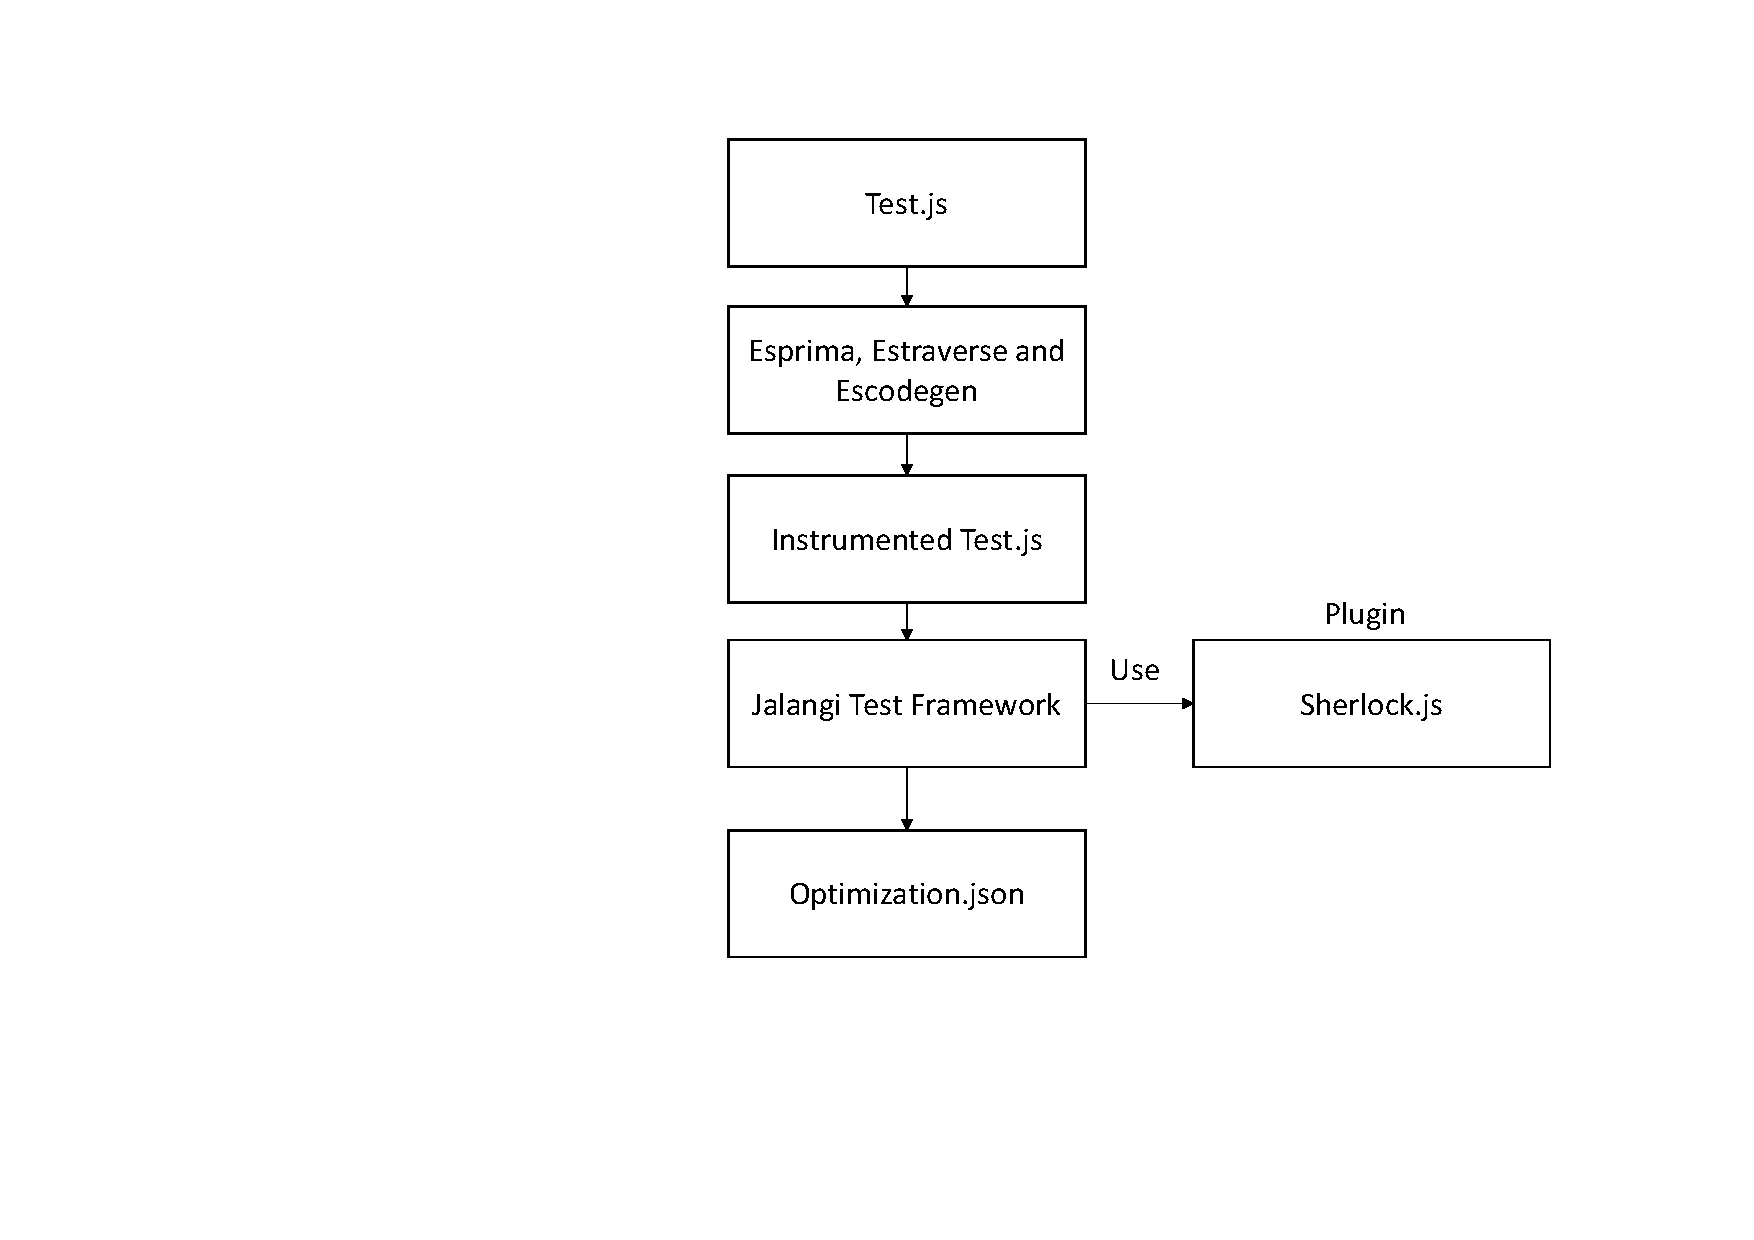
\includegraphics[width=0.8\linewidth]{architecture.png}
\captionof{figure}{Architecture of Sherlock}
\label{fig1}

\end{center}
%
%To track every object or array created during one execution, Sherlock uses a data structure called \textit{Reference}. One \textit{Reference} object may keep track of multiple references to one object/array. Furthermore Sherlock maintains some variables during the execution.
%
%\begin{itemize}
%\item{\textbf{callStack}} is an array of \js{strings} that represent the current call stack. The call stack is cleared, if \js{endExpression} is called. 
%
%\item{\textbf{allRefs}} is an array of \js{References} that the plugin tracks at the moment.
%\end{itemize}
%
%Whenever an object property or an array element is read, it cannot be optimized further. 
%In order to do this, Sherlock can lock array elements or object properties if they have been read.
\end{posterbox}

%----------------------------------------------------------------------------------------
%	REFERENCES
%----------------------------------------------------------------------------------------

\begin{posterbox}[name=references,column=0,below=methods]{References}

\smaller % Reduce the font size in this block
\renewcommand{\section}[2]{\vskip 0.05em} % Get rid of the default "References" section title
\nocite{*} % Insert publications even if they are not cited in the poster

\bibliographystyle{unsrt}
\bibliography{sample} % Use sample.bib as the bibliography file
\end{posterbox}



%----------------------------------------------------------------------------------------
%	RESULTS 
%----------------------------------------------------------------------------------------

\begin{posterbox}[name=results1,span=2,column=1,row=0]{Results} 
Sherlock was evalutad with a set of self written test-cases. The results show Sherlock is able to detect different early property optimizations. Due the fact that one goal of Sherlock was to minimize the number of false positives as low as possible, there are some cases which Sherlock does not support.\\

\textbf{Supported early property optimizations} \\ 
The cases which are fully supported by Sherlock are listed below in different code examples.

\begin{center}
\begin{tabular}{|c c |c }
\begin{lstlisting}[language=Javascript]
var a = []; 
a[0] = 1;
//optimization: var a = [1];
var b = {}; 
b.a = 5;
//optimization: var b = {a: 5};
\end{lstlisting}
& &
\begin{lstlisting}[language=Javascript]
var a =[1,2,3,4];  
a.reverse();
// optimization: var a = [4,3,2,1];
\end{lstlisting} 
\end{tabular}
\setlength{\tabcolsep}{12em}
\captionof{lstlisting}{Examples for a typical potential early property and array
element initialization}
\end{center}

The left Example shows typical potential for early property and array element initilization which is covered by Sherlock. Sherlock is also able to optimize the JavaScript built in functions for arrays (right Example).
%In order to decide which built functions it can optimize, Sherlock divide the functions in four different groups.
%
%
%\begin{itemize}
%\item{\textbf{Ignore}}
%\item{\textbf{Lock reference}}
%\item{\textbf{Call on unlocked}}
%\item{\textbf{Other}}
%\end{itemize}


In the length example the only supported optimization would be made for \textit{a}. \textit{b} must not be optimized, because this would change the semantics. \textit{c}  and \textit{d} show two corner cases that are not supported, due it is very hard to distinguish \textit{c}  and \textit{d} using Jalangi.\\
Conditioned initialization should only be done, if the scope does allow it. In the conditioned example only \textit{} can be optimized.

\begin{center}
\begin{tabular}{|l l |l }
\begin{lstlisting}[language=Javascript]
var a = [];
a[a.length] = 0;
a[1] = 1;
//optimization: var a =[0,1];
var b = [1, 2, 3];
console.log(b.length);
b[3] = 4;
//cannot be optimized
var c = [];
c[c.length - 1] = 0;
//cannot be optimized
var d = [];
d[0] = d.length - 1;
//cannot be optimized
\end{lstlisting}
& &
\begin{lstlisting}[language=Javascript]
var a = []
if (cond) {
  a[0] = 1;
  var b = []
  b[0] = 1;
	//optimization: var b =[1];
}
\end{lstlisting} 
\end{tabular}
\setlength{\tabcolsep}{12em}
\captionof{lstlisting}{Array.length and conditioned example}
\end{center}

\textbf{Not supported early property optimizations} \\ 
Some cases are not covered by Sherlock, due the fact that one of Sherlock's main goal is to keep the number of false positives as low as possible and to limit the scope of the tool. This includes objects that are created using a constructor or if a function is used in the initialization. The impact of optimization suggested by Sherlock can be seen in Figure ?.


 
\begin{center}
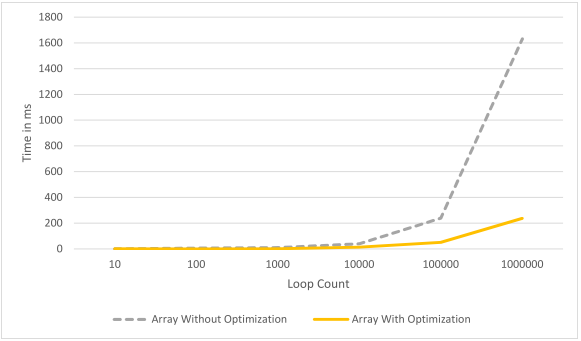
\includegraphics[width=0.7\linewidth]{impact.png}
\captionof{figure}{Benchmark for simple array initialization. Array length is 100. }
\end{center}


\end{posterbox}

%----------------------------------------------------------------------------------------
%	Conclusion
%----------------------------------------------------------------------------------------

\begin{posterbox}[name=conclusion,span=2,column=1,below=results1]{Conclusion} 
We introduced a new profiling tool to find opportunities for early property initialization, named Sherlock. While there is still a long way to go to find all possible early property optimizations our results show that Sherlock is able to find a broad range of them. Furthermore Sherlock should be able to check every JavaScript file provided to it. 

%
%Nunc sit amet sem ut nulla tincidunt mattis vel nec mauris. Vestibulum odio tellus, lobortis. Vel adipiscing, Aliquam dictum, ligula egestas commodo posuere, lectus lectus congue ligula, sed posuere urna lectus at nisi. Aenean commodo risus ut dolor (viverra scelerisque). Nullam varius, lacus et interdum hendrerit, odio orci ultrices mauris, id interdum eros mauris at urna. Fusce in nisi eros, sit amet volutpat turpis, \textbf{porttior magna} (commodo blandit euismod) \textbf{facilisis ornate magnis} (dis magnis). 
%
%%------------------------------------------------
%
%\begin{center}
%
\includegraphics[width=0.49\linewidth]{placeholder}
%
\includegraphics[width=0.49\linewidth]{placeholder}
%\captionof{figure}{Figure caption 1 (left); Figure caption 2 (right)}
%\end{center}
%
%%------------------------------------------------
%
%Aliquam ac justo lectus. Nunc ultrices aliquet purus non dictum. Nulla facilisi. Quisque vitae urna non purus sollicitudin venenatis. Aliquam erat volutpat. Cum sociis natoque penatibus et magnis dis parturient montes, nascetur ridiculus mus. In hendrerit tortor sed massa consequat eu viverra justo porta. Ut nec felis sem, non elementum.
%
%%------------------------------------------------
%
%\begin{center}
%
\includegraphics[width=0.8\linewidth]{placeholder}
%\captionof{figure}{Figure caption}
%\end{center}
%
%%------------------------------------------------
%
%Nunc sit amet sem ut nulla tincidunt mattis vel nec mauris. Vestibulum odio tellus, lobortis. Vel adipiscing, Aliquam dictum, ligula egestas commodo posuere, lectus lectus congue ligula, sed posuere urna lectus at nisi. Aenean commodo risus ut dolor (viverra scelerisque). Nullam varius, lacus et interdum hendrerit, odio orci ultrices mauris, id interdum eros mauris at urna. Fusce in nisi eros, sit amet volutpat turpis, \textbf{porttior magna} (commodo blandit euismod) \textbf{facilisis ornate magnis} (dis magnis). Aliquam ac justo lectus. Nunc ultrices aliquet purus non dictum. Nulla facilisi. Quisque vitae urna non purus sollicitudin venenatis. Aliquam erat volutpat. Cum sociis natoque penatibus et magnis dis parturient montes, nascetur ridiculus mus. In hendrerit tortor sed massa consequat eu viverra justo porta. Ut nec felis sem, non elementum.
\end{posterbox}

%----------------------------------------------------------------------------------------
%	ACKNOWLEDGEMENTS
%----------------------------------------------------------------------------------------

\begin{posterbox}[name=acknowledgements,span=2,column=1,below=conclusion]{Acknowledgements}

\smaller % Reduce the font size in this block
Fusce mattis tellus ac odio imperdiet lobortis. Cum sociis natoque penatibus et magnis dis parturient montes, nascetur ridiculus mus. Phasellus commodo blandit euismod. Ut porttitor cursus magna.
\end{posterbox}


%----------------------------------------------------------------------------------------

\end{poster}

\end{document}